\documentclass[a4paper,14pt]{extarticle}

% Путь до папки с общими шаблонами
\newcommand{\pathToCommonFolder}{/home/denilai/Documents/repos/latex/Common}
% Название работы в титуле
\newcommand{\workname}{Отчет по практической работе №4}
% Название дисциплины в титуле
\newcommand{\discipline}{Архитектура процессоров и микропроцессоров}
% Название кафедры в титуле
\newcommand{\kafedra}{Кафедра вычислительной техники}
% Тема работы в титуле
\newcommand{\theme}{Стадии выполнения команд процессором КР580ВМ80}
% Должность преподавателя в титуле
\newcommand{\rang}{cтарший преподаватель кафедры ВТ}
% ФИО преподавателя в титуле
\newcommand{\teacherfio}{Ю.~М.Скрябин}
\newcommand{\studentfio}{К.~Ю.~Денисов}
\newcommand{\signature}{\pathToCommonFolder/denisov-signature}

\newcommand{\pt}{PacketTracer\copyright}

\usepackage{tabularx}



\usepackage{booktabs}
\newcolumntype{b}{X}
\newcolumntype{s}{>{\hsize=.5\hsize}X}
\newcommand{\heading}[1]{\multicolumn{1}{|c|}{#1}}

% установка размера шрифта для всего документа
%\fontsize{20pt}{18pt}\selectfont
\usepackage{extsizes} % Возможность сделать 14-й шрифт

% Вставка заготовки преамбулы
% Этот шаблон документа разработан в 2014 году
% Данилом Фёдоровых (danil@fedorovykh.ru) 
% для использования в курсе 
% <<Документы и презентации в \LaTeX>>, записанном НИУ ВШЭ
% для Coursera.org: http://coursera.org/course/latex .
% Исходная версия шаблона --- 
% https://www.writelatex.com/coursera/latex/5.3

% В этом документе преамбула

% Для корректного использования русских символов в формулах
% пакеты hyperref и настройки, связанные с ним, стоит загуржать
% перед загрузкой пакета mathtext



% поддержка русских букв
% кодировка шрифта
%\usepackage[T2A]{fontenc} 
\usepackage{pscyr}

% использование ненумеровонного абзаца с добавлением его в содержаниеl

\newcommand{\anonsection}[1]{\section*{#1}\addcontentsline{toc}{section}{#1}}
\newcommand{\sectionunderl}[1]{\section*{\underline{#1}}}


% настройка окружения enumerate
\usepackage{enumitem}
\setlist{noitemsep}
\setlist[enumerate]{labelsep=*, leftmargin=1.5pc}

\usepackage{hyperref}

% сначала ставить \usepackage{extsizes} % Возможность сделать 14-й шрифт
% для корректной установки полей вставлять преамбулу следует в последнюю очередь (но перед дерективой замены \rmdefault)
\usepackage[top=20mm,bottom=25mm,left=35mm,right=20mm]{geometry} % Простой способ задавать поля

\hypersetup{				% Гиперссылки
	unicode=true,           % русские буквы в раздела PDF
	pdftitle={Заголовок},   % Заголовок
	pdfauthor={Автор},      % Автор
	pdfsubject={Тема},      % Тема
	pdfcreator={Создатель}, % Создатель
	pdfproducer={Производитель}, % Производитель
	pdfkeywords={keyword1} {key2} {key3}, % Ключевые слова
	colorlinks=true,       	% false: ссылки в рамках; true: цветные ссылки
	linkcolor=red,          % внутренние ссылки
	citecolor=black,        % на библиографию
	filecolor=magenta,      % на файлы
	urlcolor=blue           % на URL
}

%%% Работа с русским языком
\usepackage{cmap}					% поиск в PDF
\usepackage{mathtext} 				% русские буквы в формулах
\usepackage[T2A]{fontenc}			% кодировка
\usepackage[utf8]{inputenc}			% кодировка исходного текста
\usepackage[english,russian]{babel}	% локализация и переносы
\usepackage{indentfirst}
\frenchspacing

%для изменения названия списка иллюстраций
\usepackage{tocloft}


\renewcommand{\epsilon}{\ensuremath{\varepsilon}}
\renewcommand{\phi}{\ensuremath{\varphi}}
\renewcommand{\kappa}{\ensuremath{\varkappa}}
\renewcommand{\le}{\ensuremath{\leqslant}}
\renewcommand{\leq}{\ensuremath{\leqslant}}
\renewcommand{\ge}{\ensuremath{\geqslant}}
\renewcommand{\geq}{\ensuremath{\geqslant}}
\renewcommand{\emptyset}{\varnothing}

% Изменения параметров списка иллюстраций
\renewcommand{\cftfigfont}{Рисунок } % добавляем везде "Рисунок" перед номером
\addto\captionsrussian{\renewcommand\listfigurename{Список иллюстративного материала}}

\newcommand{\tm}{\texttrademark\ }
\newcommand{\reg}{\textregistered\ }


%%% Дополнительная работа с математикой
\usepackage{amsmath,amsfonts,amssymb,amsthm,mathtools} % AMS
\usepackage{icomma} % "Умная" запятая: $0,2$ --- число, $0, 2$ --- перечисление

%% Номера формул
%\mathtoolsset{showonlyrefs=true} % Показывать номера только у тех формул, на которые есть \eqref{} в тексте.
%\usepackage{leqno} % Нумереация формул слева

%% Свои команды
\DeclareMathOperator{\sgn}{\mathop{sgn}}

%% Перенос знаков в формулах (по Львовскому)
\newcommand*{\hm}[1]{#1\nobreak\discretionary{}
{\hbox{$\mathsurround=0pt #1$}}{}}


% отступ для первого абзаца главы или параграфа
%\usepackage{indentfirst}

%%% Работа с картинками
\usepackage{graphicx}  % Для вставки рисунков
\graphicspath{{images/}{screnshots/}}  % папки с картинками
\DeclareGraphicsExtensions{.pdf,.png,.jpg}
\setlength\fboxsep{3pt} % Отступ рамки \fbox{} от рисунка
\setlength\fboxrule{1pt} % Толщина линий рамки \fbox{}
\usepackage{wrapfig} % Обтекание рисунков текстом

%%% Работа с таблицами
\usepackage{array,tabularx,tabulary,booktabs} % Дополнительная работа с таблицами
\usepackage{longtable}  % Длинные таблицы
\usepackage{multirow} % Слияние строк в таблице

%%% Теоремы
\theoremstyle{plain} % Это стиль по умолчанию, его можно не переопределять.
\newtheorem{theorem}{Теорема}[section]
\newtheorem{proposition}[theorem]{Утверждение}

\theoremstyle{plain} % Это стиль по умолчанию, его можно не переопределять.
\newtheorem{work}{Практическая работа}[part]


 
 
\theoremstyle{definition} % "Определение"
\newtheorem{corollary}{Следствие}[theorem]
\newtheorem{problem}{Задача}[section]
 
\theoremstyle{remark} % "Примечание"
\newtheorem*{nonum}{Решение}



%%% Программирование
\usepackage{etoolbox} % логические операторы

%%% Страница

%	\usepackage{fancyhdr} % Колонтитулы
% 	\pagestyle{fancy}
%   \renewcommand{\headrulewidth}{0pt}  % Толщина линейки, отчеркивающей верхний колонтитул
% 	\lfoot{Нижний левый}
% 	\rfoot{Нижний правый}
% 	\rhead{Верхний правый}
% 	\chead{Верхний в центре}
% 	\lhead{Верхний левый}
%	\cfoot{Нижний в центре} % По умолчанию здесь номер страницы

\usepackage{setspace} % Интерлиньяж
\onehalfspacing % Интерлиньяж 1.5
%\doublespacing % Интерлиньяж 2
%\singlespacing % Интерлиньяж 1

\usepackage{lastpage} % Узнать, сколько всего страниц в документе.

\usepackage{soul} % Модификаторы начертания


\usepackage[usenames,dvipsnames,svgnames,table,rgb]{xcolor}


\usepackage{csquotes} % Еще инструменты для ссылок

%\usepackage[style=authoryear,maxcitenames=2,backend=biber,sorting=nty]{biblatex}

\usepackage{multicol} % Несколько колонок

\usepackage{tikz} % Работа с графикой
\usepackage{pgfplots}
\usepackage{pgfplotstable}

% модуль для вставки рыбы
\usepackage{blindtext}

\usepackage{listings}
\usepackage{color}


% для поворота отдельной страницы. Использовать окружение \landscape
\usepackage{pdflscape} 
\usepackage{rotating} 


\definecolor{mygreen}{rgb}{0,0.6,0}
\definecolor{mygray}{rgb}{0.5,0.5,0.5}
\definecolor{mymauve}{rgb}{0.58,0,0.82}


% пример импорта файла
%\lstinputlisting{/home/denilai/repomy/conf/distributions}

\lstset{
	language=Python,
	basicstyle=\footnotesize,        % the size of the fonts that are used for the code
	numbers=left,                    % where to put the line-numbers; possible values are (none, left, right)
	numbersep=5pt,                   % how far the line-numbers are from the code
	numberstyle=\tiny\color{mygray}, % the style that is used for the line-numbers
	stepnumber=2,                    % the step between two line-numbers. If it's 1, each line will be numbered
	% Tab - 2 пробела
	tabsize=2,    
	% Автоматический перенос строк
	breaklines=true,
	frame=single,
	breakatwhitespace=true,
	title=\lstname 
}



\author{Кирилл Денисов ИВБО-02-19}
\title{Практическая работа №5\\Вариант 6}
\date{\today}

\renewcommand{\withouttheme}{1}

% установка полуторного интервала
% \usepackage{setspace}  
% \onehalfspacing

% использовать Times New Roman
\renewcommand{\rmdefault}{ftm}


\begin{document}
	%\thispagestyle{empty}
	% Вставка первого титульного листа
	%%\newcommand{\withouttheme}{} добавить эту переменную для определения, нужна ли тема
%     {} - нужна
%    {1} - не нужна

%\newcommand{\withoutsubmissiondate}{} добавить эту переменную для определения, нужен ли срок предоставления отчета
%     {} - нужен
%    {1} - не нужен
\begin{center}
	\begin{figure}[h!]
		\begin{center}
		
\includegraphics[width=0.17\linewidth]{\pathToCommonFolder/gerb}
		%\caption{}\label{pic:first}
		%	\vspace{5ex}
		\end{center}	
	\end{figure}
 	\small	МИНОБРНАУКИ РОССИИ \\
	Федеральное государственное бюджетное образовательное учреждение\\
						высшего профессионального образования\\
\normalsize					
\textbf{«МИРЭА – Российский технологический университет»\\
						РТУ МИРЭА}\\
						\noindent\rule{1\linewidth}{1pt}\\
       Институт информационных технологий\\ %\vspace{2ex}
					\kafedra\\
		\vspace{3ex}
			\large \textbf{\workname}  \\
		%\vspace{1ex}
						по дисциплине\\ «\discipline» \\
		\vspace{3ex}
		\if \withouttheme
			\textbf{Тема работы:}\\ <<\theme>>
		\fi
\vspace{3ex}
\small
\begin{table}[h!]
\begin{tabular}{p{0.14\linewidth}p{0.38\linewidth}p{0.25\linewidth}p{0.2\linewidth}}
	\textbf{Выполнил:} & студент группы ИВБО-02-19 & \studentfio &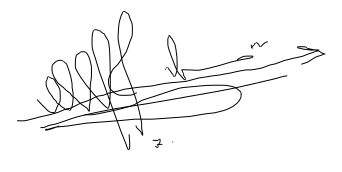
\includegraphics[width=0.8\linewidth]{\signature}\\ \\
	\textbf{Принял:} & \rang & \teacherfio 
\end{tabular}
\end{table}
\end{center}

\begin{flushleft}
	\begin{tabular}{p{0.25\linewidth}l}

		Работа выполена & <<\noindent\rule{2em}{1pt}>>
		                    \noindent\rule{5em}{1pt} 202\noindent\rule{1em}{1pt} \\

		<<Зачтено>> & <<\noindent\rule{2em}{1pt}>>
		\noindent\rule{5em}{1pt} 202\noindent\rule{1em}{1pt} \\

	\end{tabular}
\end{flushleft}

\normalsize
\begin{center}	
\vfill 
Москва 2021
\end{center}

	\newpage
	%\tableofcontents
	\newpage
	%\listoftables
\maketitle


\begin{table}[htbp]
\begin{center}
		\caption{Таблица адресации}
	\begin{tabular}{|p{0.17\linewidth}|l|l|l|p{0.2\linewidth}|}
		\hline
		Устройство  & Интерфейс & IP-адрес & Маска подсети & Шлюз по умолчанию \\ \hline
		\multirow{2}{*}{R1\_DENISOV} & G0/0 & 192.168.6.1 & 255.255.255.0 & --- \\ \cline{2-5}
		                            & G0/0 & 192.168.7.1 & 255.255.255.0 & --- \\ \hline
		PC-A & NIC & 192.168.7.3 & 255.255.255.0 & 192.168.7.1 \\ \hline
		PC-B & NIC & 192.168.6.3 & 255.255.255.0 & 192.168.6.1 \\ \hline
	\end{tabular}
	\label{tab:adress}
\end{center}
\end{table}

\begin{mypart}{Настройка топологии и инициализация устройств}
\step{Создание сети согласно топологии}

Построим локальную сеть переименовав устройства в соответствии с вариантом задания (см. рисунок \ref{fig:pract5-topology}).

% TODO: \usepackage{graphicx} required
\begin{figure}[htbp]
	\centering
	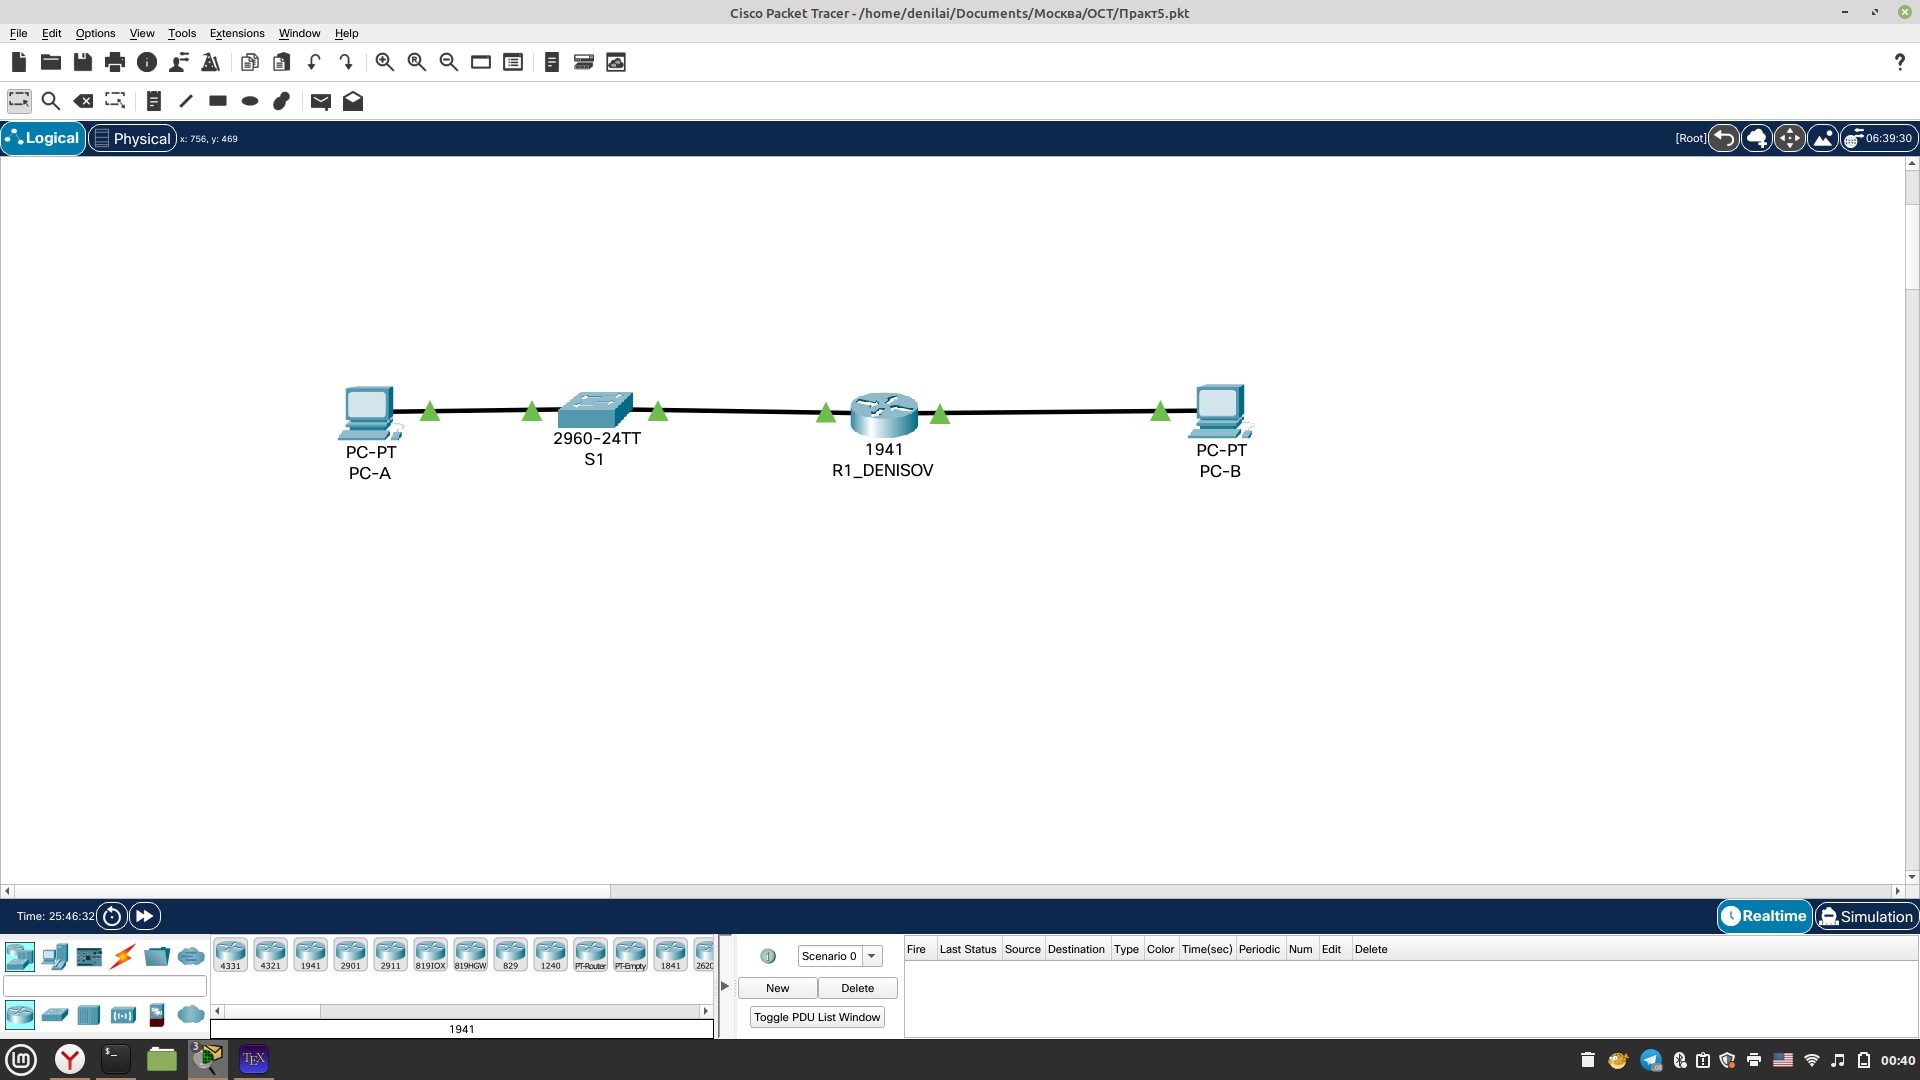
\includegraphics[width=0.5\linewidth]{images/pract5-topology}
	\caption{Топология сети}
	\label{fig:pract5-topology}
\end{figure}
\end{mypart}
\newpage
\begin{mypart}{Настройка устройств и проверка подключения}

\step{Статическая настройка IP-адресации на ПК}

Настроим IP-адресы на PC в соответствии с таблицей адресации \ref{tab:adress} (см. рисунки \ref{fig:pract5-pc-a-ip}, \ref{fig:pract5-pc-b-ip1}).

% TODO: \usepackage{graphicx} required
\begin{figure}[h!]
	\centering
	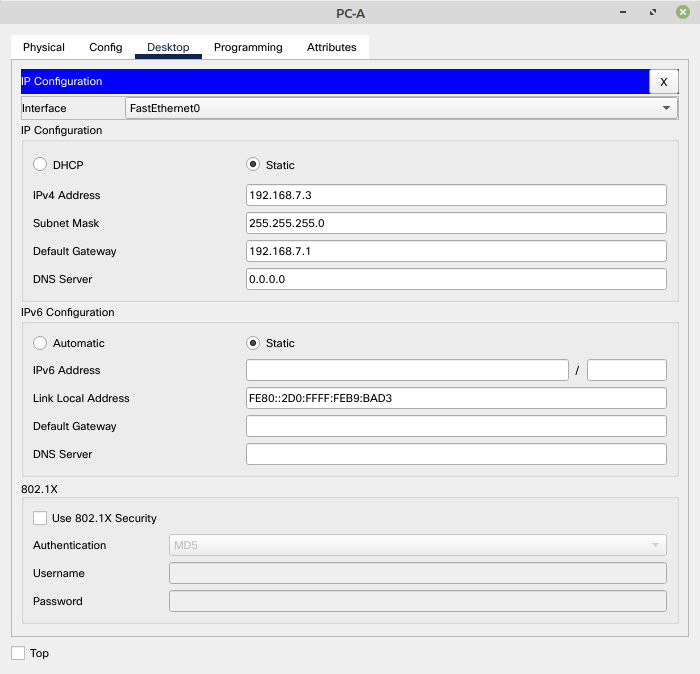
\includegraphics[width=0.4\linewidth]{images/pract5-pc-a-ip}
	\caption{IP-адрес PC-A}
	\label{fig:pract5-pc-a-ip}
\end{figure}

% TODO: \usepackage{graphicx} required
\begin{figure}[h!]
	\centering
	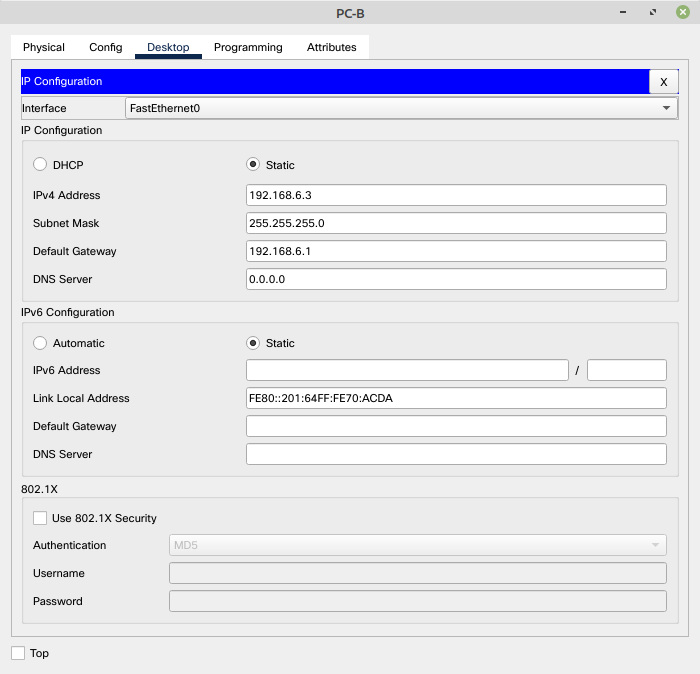
\includegraphics[width=0.4\linewidth]{images/pract5-pc-b-ip1}
	\caption{IP-адрес PC-B}
	\label{fig:pract5-pc-b-ip1}
\end{figure}

Отправим эхо-запрос на PC-B из командной строки PC-A (см. рисунок~\ref{fig:pract5-ping}). Запрос не был доставлен, потому что маршрутизатор R1\_DENISOV не настроен.

% TODO: \usepackage{graphicx} required
\begin{figure}[h!]
	\centering
	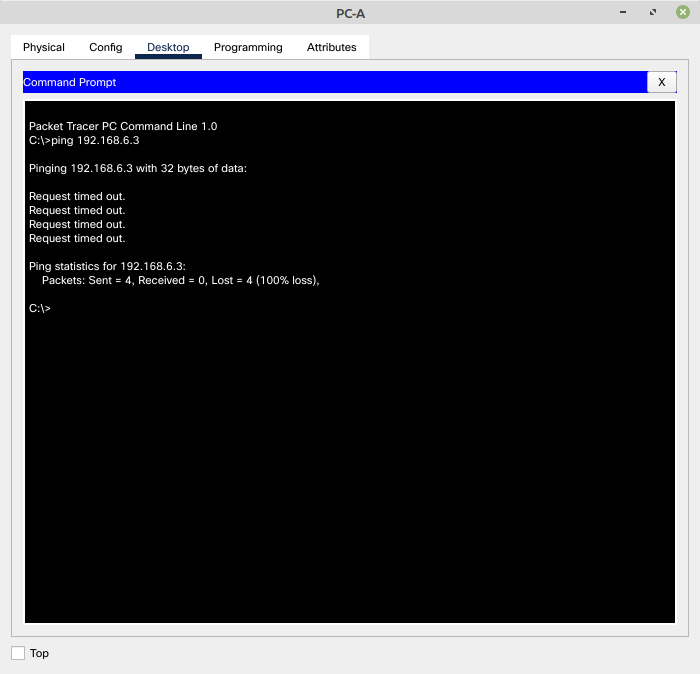
\includegraphics[width=0.5\linewidth]{images/pract5-ping}
	\caption{Эхо-запрос c PC-A до PC-B }
	\label{fig:pract5-ping}
\end{figure}

\step{Настройка маршрутизатора}

Произведем все указанные шаги по первоначальной настройке маршрутизатора Cisco 1941.

Результат работы вызова команды \texttt{show running-config} приведен в листинге.
\newpage

\begin{lstlisting}
	R1_DENISOV#show running-config 
	Building configuration...
	
	Current configuration : 874 bytes
	!
	version 15.1
	no service timestamps log datetime msec
	no service timestamps debug datetime msec
	service password-encryption
	!
	hostname R1_DENISOV
	!
	enable secret 5 $1$mERr$9cTjUIEqNGurQiFU.ZeCi1
	!
	ip cef
	no ipv6 cef
	!
	license udi pid CISCO1941/K9 sn FTX1524P0OU-
	!
	no ip domain-lookup
	!
	spanning-tree mode pvst
	!
	interface GigabitEthernet0/0
	description connecting to pc-b
	ip address 192.168.6.1 255.255.255.0
	duplex auto
	speed auto
	!
	interface GigabitEthernet0/1
	description connecting to S1
	ip address 192.168.7.1 255.255.255.0
	duplex auto
	speed auto
	!
	interface Vlan1
	no ip address
	!
	ip classless
	!
	ip flow-export version 9
	!
	banner motd ^CAuthorization access only!^C
	!
	!
	line con 0
	password 7 0822455D0A16
	login
	!
	line aux 0
	!
	line vty 0
	password 7 0822455D0A16
	login
	line vty 1 4
	login
	!
	end
\end{lstlisting}

Протестируем компьютер PC-B, отправив компьютеру PC-A эхо-запрос из окна командной строки.
Проверка связи выполнена успешно, потому что маршрутизатор направил ICMP пакет из одной подсети в другую и обратно.

Результаты работы команды ping приведены на рисунке \ref{fig:pract5-ping2}.

% TODO: \usepackage{graphicx} required
\begin{figure}[h!]
	\centering
	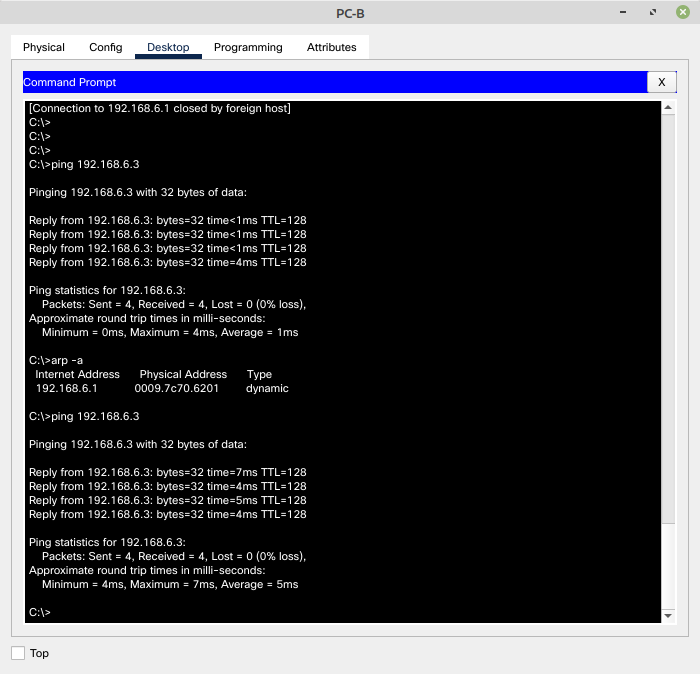
\includegraphics[width=0.5\linewidth]{images/pract5-ping2}
	\caption{Эхо-запрос c PC-B до PC-A}
	\label{fig:pract5-ping2}
\end{figure}
\end{mypart}
\begin{mypart}{Отображение сведений об устройстве}

\step{Сбор данных об аппаратном и программном обеспечении с сетевых устройств}

С помощью команды \texttt{show version}, выполненной в командной строке маршрутизатора R1\_DENISOV ответим на следующие вопросы:
\begin{enumerate}
	\item Как называется образ IOS, под управлением которой работает маршрутизатор?
		\\\textbf{Ответ:} flash0:c1900-universalk9-mz.SPA.151-1.M4.bin
	\item Каким объемом памяти DRAM обладает маршрутизатор?
		\\\textbf{Ответ:} 32 МБ
	\item Каким объемом памяти NVRAM обладает маршрутизатор?
		\\\textbf{Ответ:} 255 КБ
	\item Каким объемом флеш-памяти обладает маршрутизатор?
		\\\textbf{Ответ:} 249856 КБ
	
\end{enumerate}

С помощью команды \texttt{show version}, выполненной в командной строке коммутатора S1 ответим на следующие вопросы:
\begin{enumerate}
	\item Как называется образ IOS, под управлением которой работает коммутатор?
		\\\textbf{Ответ:} Не указана
	\item Каким объемом динамического ОЗУ (DRAM) обладает коммутатор?
		\\\textbf{Ответ:} 21039 КБ
	\item Каким объемом энергонезависимой памяти (NVRAM) обладает коммутатор?
		\\\textbf{Ответ:} 63488 КБ
	\item Назовите номер модели коммутатора
		\\\textbf{Ответ:} WS-C2960-24TT-L
\end{enumerate}

\step{Отображение таблицы маршрутизации на маршрутизаторе}

Выполним команду \texttt{show ip route} в командной строке маршрутизатора R1\_DENISOV, чтобы ответить на следующие вопросы:
\begin{enumerate}
	\item Какой код используется в таблице маршрутизации для обозначения сети с прямым подключением?
		\\\textbf{Ответ:} <<C>>
	\item Сколько записей маршрутов обозначены буквой «C» в таблице маршрутизации?
		\\\textbf{Ответ:} 2
	\item Какие типы интерфейсов связаны с маршрутами, закодированными с символом «C»?
		\\\textbf{Ответ:} GigabitEthernet
\end{enumerate}
Таблица маршрутизации также приведена на рисунке \ref{fig:pract5-ip-route}.
% TODO: \usepackage{graphicx} required
\begin{figure}[h!]
	\centering
	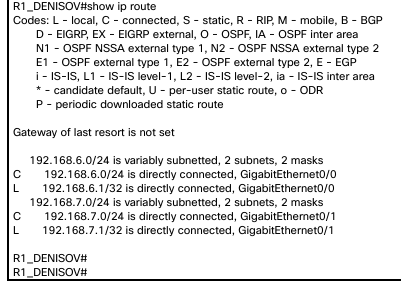
\includegraphics[width=0.4\linewidth]{images/pract5-ip-route}
	\caption{Таблица маршрутизации R1\_DENISOV}
	\label{fig:pract5-ip-route}
\end{figure}

\step{Выведение на маршрутизатор сведения об интерфейсе}

С помощью команды \texttt{show interface g0/1} ответим на следующие вопросы:
\begin{enumerate}
	\item Укажите текущее состояние интерфейса G0/1
		\\\textbf{Ответ:} GigabitEthernet0/1 is up, line protocol is up (connected)
	\item Назовите МАС-адрес интерфейса G0/1.
		\\\textbf{Ответ:} (bia 0009.7c70.6202)
	\item Каким образом в этой команде отображается адрес в Интернете?
		\\\textbf{Ответ:} Internet address is 192.168.7.1/24
\end{enumerate}

\step{Выведение на маршрутизатор и коммутатор сводный список интерфейсов}

Для проверки конфигурации интерфейса существует несколько команд. Самая удобная --- команда \texttt{show ip interface brief}. Выходные данные команды содержат сводный список интерфейсов устройства с указанием статуса каждого интерфейса. 

Результат работы команды \texttt{show ip interface brief} на маршрутизаторе R1\_DENISOV приведен на рисунке \ref{fig:pract5-ip-interface}.
% TODO: \usepackage{graphicx} required
\begin{figure}[h!]
	\centering
	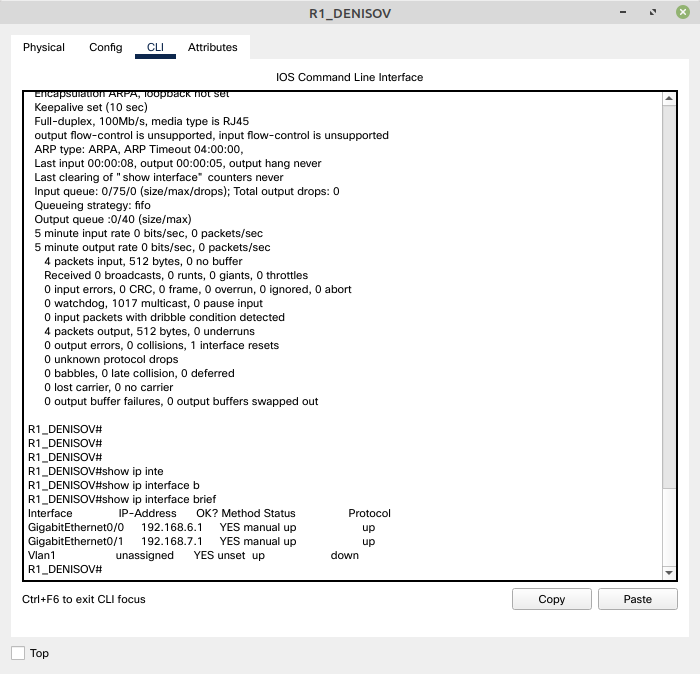
\includegraphics[width=0.5\linewidth]{images/pract5-ip-interface}
	\caption{вывод команды \texttt{show ip interface brief} на R1\_DENISOV}
	\label{fig:pract5-ip-interface}
\end{figure}

Результат работы команды \texttt{show ip interface brief} на коммутаторе S1 приведен на рисунке \ref{fig:pract5-ip-interface-s1}.

% TODO: \usepackage{graphicx} required
\begin{figure}[h!]
	\centering
	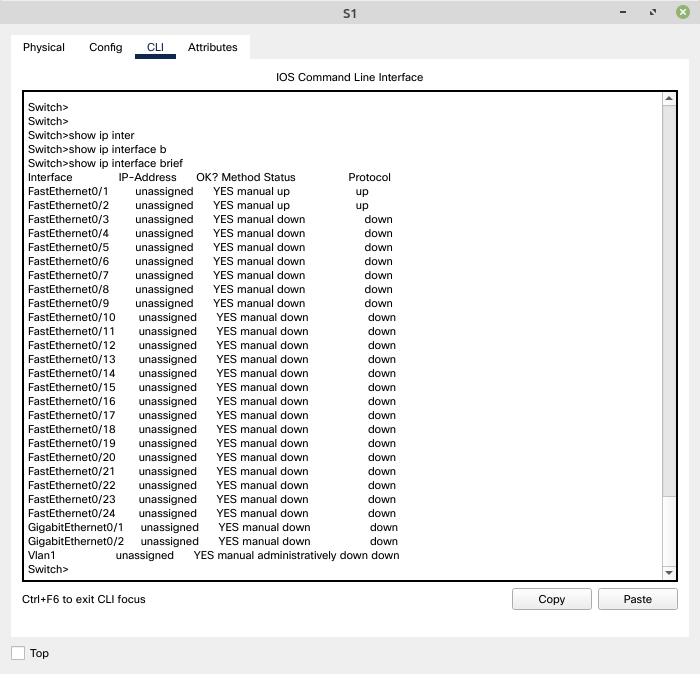
\includegraphics[width=0.5\linewidth]{images/pract5-ip-interface-s1}
	\caption{вывод команды \texttt{show ip interface brief} на S1}
	\label{fig:pract5-ip-interface-s1}
\end{figure}
\end{mypart}
\begin{mypart}{Защита лабораторной работы (ответ на контрольные
	вопросы и вопросы преподавателя)}


\begin{enumerate}
	\item Если интерфейс G0/1 выключен администратором, какая команда конфигурации интерфейса позволит
	его включить?
		\\\textbf{Ответ:} no shutdown
	\item Что произойдет в случае неправильной конфигурации интерфейса G0/1 на маршрутизаторе с IP-адресом 192.168.7.1?
		\\\textbf{Ответ:} Пакеты с конечного узла PC-A не смогу покинуть пределы подсетей источника, потому что адрес 192.168.1.1 является для них основным шлюзом~---~механизмом передачи пакетов в удаленные сети.
\end{enumerate}

\end{mypart}

\end{document}



